%!TEX root = thesis.tex

\renewcommand{\TheTitle}{Influence of Multiple Firebrands on the Ignition of Fuel Beds}
\renewcommand{\TheAuthors}{Derek Bean, David L. Blunck \\ \\ My contributions to this work included the design of the experiments, fabrication of the experimental apparatus, collecting data, data analysis, conducting part of the modelling efforts, and preparation of the manuscript.}

\renewcommand{\TheAddress}{
\textbf{Status: In Preparation}
}

\PaperHeader{\TheTitle}{\TheAuthors}{\TheAddress}

\chapter{\TheTitle}
\label{part:manuscript4}

\section{Abstract}
    some text
\section{Introduction}
    The combination of increasing wildfire severity and an increase of homes in the Wildland Urban Interface (WUI) has significantly increased the occurrence of home loss due to wildfires since the turn of the century~\cite{Manzello2013}. Ignition of fuels by firebrands that leads to the loss of a structure is a primary source of home loss~\cite{Koo2010a, Syphard2019, Roberts2021}, and in some fires has been the source of 2/3 of structure ignitions~\cite{Maranghides2013NISTIgnitions}. Thus, it is important to understand the ignition of fuel beds by firebrands in order to mitigate the risk of ignition~\cite{Manzello2014}. Ideally, the understanding of the ignition process would result in a predictive model that would enable homeowners, firefighters, and other risk management personnel to determine location specific strategies for preventing ignition before and during a fire. Unfortunately, such a model does not currently exist due to critical shortfalls in the current knowledge of fuel bed ignition. 
    
    Processes that influence ignition begin within the fire when an ember (e.g., branch, bark, cone etc) is ignited and lofted into the air by wind. The combusting ember is then transported to and lands on a fuel bed near or on a structure. Energy is then transferred to the fuel bed and if the energy is sufficient the fuel bed will undergo pyrolysis and produce flammable gases which may then ignite and begin flaming. These flames may then spread and destroy the structure. Each of these processes, ember generation, transport, and ignition, require additional research before a predictive model is possible. This work focuses on the processes that occur during ignition of the fuel bed.
    
    An additional risk factor for the ignition of structures is the accumulation of embers on fuel beds. The geometry of homes often promotes the accumulation of embers by creating recirculation zones which promote the deposition of embers. The accumulation of embers poses an increased risk of home ignition in multiple ways. First, since ignition is largely a stochastic process, the more embers that land on an area the larger the probability of ignition. Second, embers that accumulate close to one another creating piles may depart more energy onto a fuel bed than a single ember alone. In work conducted by Hakes et al.~\cite{Hakes2019a} an increase in firebrand pile mass increased the total energy imparted to an instrumented surface. The increase in energy release was attained by a longer duration of energy release as the pile mass increased.
    
    The accumulation of embers near structures also requires the presence of wind which has also been shown to influence ignition. The presence of wind has been shown to decrease the threshold of ignition. In work conducted by Suzuki and Manzello~\cite{Suzuki2020a} when wind was increased from 6\si{\meter\per\second} to 8\si{\meter\per\second} the number of embers required for ignition of the wood much fuel bed decreased. Similar observations of wind lowering the ignition threshold have been observed in multiple studies with single embers. Wang et al.~\cite{Wang2017} reported decreases in ignition times as wind speed increased for hot metal particles dropped on pine needle fuel beds. Ellis reported that the addition of wind increased the threshold of fuel moisture content where ignition was observed for natural firebrands  deposited on eucalypt forest litter. The trends observed by Ellis agreed with those observed by Ganteaume et al.~\cite{Ganteaume2009} and Pulcinski and Anderson~\cite{Plucinski2008} where the addition of wind increased ignition probability. From these studies an increase of wind increases the danger of fuel bed ignition near homes but the mechanism(s) that cause the increased ignition probability are unclear. 
    
    For single firebrands it has been postulated that the primary enhancement of wind is due to increased oxygen to the ember and fuel bed. From these works it was unclear if the ignition enhancement was due to increased heat release from the ember, increased mixing and oxygen in the pyrolyzates, or some combination of both. Results from the work outlined in Chapter~\ref{part:manuscript2} show that in the presence of an ignition source where the heat release is not influenced by wind an increase of wind increases the ignition probability. The increase in ignition probability was attributed to the accumulation of pyrolysis products near the energy source (cartridge heater) suggesting that fluid flow near the ember is a significant controlling parameter for ignition. 
    
    The addition of multiple firebrands in close proximity adds additional layers of complexity with respect to both heat release and fluid dynamics.  Hakes et al.~\cite{Hakes2019a} identified re-radiation and reheating as key processes that differentiate single embers from multiple embers and have significant influence on energy deposited to the fuel bed.  The presence of multiple embers may also create disturbances in the fluid flow around the embers that influence recirculation zones and alter the ignition propensity. What is unclear from these conclusions is the magnitude of the effect that re-radiation and flow disturbances have on ignition. Understanding the magnitude of these processes on the probability of ignition is imperative to creating accurate ignition models. 
    
    With this background and motivation, the objective of this study is to quantify the influence of multiple embers on the ignition propensity of a fuel bed. It is anticipated that the results of this work will help further the understanding of the difference in ignition propensity between a single ember and multiple embers that may interact through fluid and thermal processes. A more complete understanding of these processes will enable an increased accuracy of ignition models and better protection of structures in the WUI.
    
    
\section{Methodology}
    The probability of flaming ignition for fuel beds consisting of Douglas-fir particles was measured for eight configurations of two embers in a wind tunnel. The wind tunnel was operated at either 0.5 \si{\meter\per\second} or 5.8 \si{\meter\per\second} for each test series. The wind speed was measured with a TSI-IFA300 hot wire probe. Figure~\ref{fig:multiHeaterApparatus} shows a representation of the wind tunnel, fuel bed, and the automated lowering device. Table~\ref{tab:multiHeaterConfig} shows the test matrix for each series of tests. For all of the tests the heaters were oriented perpendicular to the flow and the downstream heater was heated. For tests where both heaters were heated the temperatures of both heaters were maintained at the same temperature. 
    
    The combinations of heater spacing and hot or ambient upstream heater were chosen to represent different levels of fluid and thermal interactions between the heaters and the fuel bed. The heater spacing of five diameters was chosen such that minimal interaction between the heaters occurs as previous CFD calculations indicate that the recirculation zone of the upstream heater is approximately five diameters when the heater is in a wind of 5.8 \si{\meter\per\second} and an orientation perpendicular to the flow. Preliminary thermal calculations also indicated that the pyrolysis fronts created by each heater are unlikely to interact within previously observed times to ignition. The heater spacing of one diameter was chosen for a high level of interaction between both the fluid disturbances and thermal fronts of each ember. The one diameter spacing places the downstream heater inside the recirculation zone of the upstream heater under wind and the preliminary heat transfer calculations indicated that the thermal fronts of each heater will merge before the anticipated time to ignition. The chosen heater orientations also represent potential scenarios that may be encountered in a wildfire. The configuration with two heaters both heated is representative of a multi ember attack where the one diameter spacing approximates a firebrand pile and the five diameter spacing approximates two embers falling in close proximity but not within each others region of influence. The configuration with only the downstream heater heated is representative of an ember falling near an object (e.g., twig, rock, or cone) that disturbs the flow and may act as a heat sink for the energy deposited to the ember with the one and five diameter spacing representing an ember falling both within and outside of the region of influence of the ember. The configuration where the upstream heater is not heated and five diameters is also considered a control for comparison to previous single heater ignition results.
    
            \rowcolors{2}{gray!25}{white}
        \begin{table}[hpbt]
            \normalsize
            \caption{Test matrix}
            \centering
            \begin{tabular}{ccccr}
                \rowcolor{gray!50}
               Test Series & Heater Spacing & Upstream Heater & U\textsubscript{bulk} (\si{\meter\per\second})\\
                \hline
                1   & 1 & Ambient & 0.5 \\
                2   & 1 & Ambient & 5.8 \\
                3   & 1 & Hot     & 0.5 \\
                4   & 1 & Hot     & 5.8 \\
                5   & 5 & Ambient & 0.5 \\
                6   & 5 & Ambient & 5.8 \\
                7   & 5 & Hot     & 0.5 \\
                8   & 5 & Hot     & 5.8 \\
            \end{tabular}
            \label{tab:multiHeaterConfig}
        \end{table}
    
    The cartridge heaters used had diameters of 6.4\si{\milli\meter} and lengths of 51\si{\milli\meter}. The heater sizes were chosen to represent large firebrands with a high potential to ignite a fuel bed in a wildfire~\cite{Manzello2007}. The heater temperatures were controlled using a PID temperature controller implemented in LabVIEW. Heater temperatures ranged from 250\si{\celsius} to 750\si{\celsius}. Heater temperatures were measured using a type-K thermocouple attached to the center of each heater opposite the fuel bed.
    Controlling the temperature of the heater provides an advantage over natural burning or smoldering embers and pre-heated particles by removing the temperature variability of the heat source and enabling real time data logging of the heat source temperature. Controlling the temperature of the ember also removes some complexity of calculating the energy imparted to the fuel bed. The heater was lowered onto the fuel bed with an automated lowering device. The lowering device included a load cell and a PID controller to maintain a force equivalent to a two 10\si{\gram} firebrands throughout the experiment. To minimize flow disruptions due to apparatus the heaters were each attached to two 4-40 threaded rods that extended approximately 100\si{\milli\meter} below the load cell. 
    
         \begin{figure}[hbpt]
            \centering
            \resizebox{0.5\columnwidth}{!}{%
                \begin{tikzpicture}
                    \filldraw[pattern=north west lines, pattern color=brown, thick] (2.84, 0)  rectangle (4.34, -.75) node[pos=0.5,rectangle,fill=white] {\scriptsize Fuel Bed};
                    \fill [draw=white,  inner color=red, outer color=white ] (3.43, 0.01) circle (0.15);
                    \fill [draw=white,  inner color=red, outer color=white ] (3.74, 0.01) circle (0.15);
                    \filldraw[draw=black,fill=white, thick] (0, 0)      rectangle (6, 3);
                    \fill[fill=black!50] (3.41, 0) rectangle (3.44, 1.40);
                    \fill[fill=black!50] (3.72, 0) rectangle (3.75, 1.40);
                    \fill[fill=black] (3.55, 1.52) rectangle (4.23, 1.57);
                    \fill[fill=black] (3.55, 1.45) rectangle (3.60, 1.52);
                    \filldraw[draw=black, fill=black!50] (3.3, 1.40) rectangle (3.86, 1.45);
                    \filldraw[draw=black, fill=black!50] (4.09, 1.57) rectangle (4.22, 3);
                   
                    \draw [<-] (3.5, 0.1) -- (3, 0.5) node[left] {\scriptsize Heater};
                    \draw [<-] (3.5, 1.55) -- (3, 1.55) node[left] {\scriptsize Load Cell};
                    \draw [<-] (3.75, 2.5) -- (3, 2.5) node[left] {\scriptsize Lowering Arm};
                    \draw[->]         (0.1, 0.6) -- (0.75, 0.6);
                    \draw[->]         (0.1, 1.2) -- (0.75, 1.2);
                    \node[right] at (-0.75, 1.5) {\scriptsize Inlet};
                    \draw[->]         (0.1, 1.8) -- (0.75, 1.8);
                    \draw[->]         (0.1, 2.4) -- (0.75, 2.4);
                    \draw[draw=black, dashed] (3.336, 0) rectangle (4.54, 0.34);
                    \draw[->]         (4.3, 1) -- (4.0, 0.34);
                    \node[right, align=left] at (4.3, 1) {\scriptsize Computational\\ \scriptsize Domain};
                    \fill[draw=red, fill=red] (3.43, 0.01) circle (0.0635);
                    \fill[draw=red, fill=red] (3.74, 0.01) circle (0.0635);
                \end{tikzpicture}
                }
            \caption{Diagram of the experimental wind tunnel apparatus. Air flows through the wind tunnel from left to right. The dashed region represents the domain subset used for computational efforts.}
            \label{fig:multiHeaterApparatus}
        \end{figure}
    
    The fuel bed material was processed from kiln dried Douglas-fir lumber. The lumber was first planed to generate shavings. The wood shavings were then granulated and screened such that the particles passed through a 2.3\si{\milli\meter} screen but not through a 1.3\si{\milli\meter} screen. The particles were then dried in an oven at 103\si{\celsius} to remove any remaining moisture content. During tests, the fuel was placed in a 140\si{\milli\meter} diameter glass container with a depth of 70\si{\milli\meter} and then inserted into the wind tunnel. The average density of the fuel beds was XX.X\si{\kilo\gram\per\cubic\meter}.
    
\section{Results and Discussion}
    The flaming ignition or non-ignition result of each test is shown in Figure~\ref{fig:multi_heater_hot_vs_ambient}. The markers show the result of each test and the the curves show the logistic regression for each of the heater configurations as defined in Table\ref{tab:multiHeaterConfig} (i.e., tests with the same wind speed, heater spacing, and upstream heater hot or ambient). The shaded regions around the curves represent the 95\% confidence intervals of each regression. The top plot in Figure~\ref{fig:multi_heater_hot_vs_ambient} shows configurations where the downstream heater is actively heated and the upstream heater is at ambient conditions. The bottom plot in Figure~\ref{fig:multi_heater_hot_vs_ambient} shows results for configurations where both heaters are actively heated to the same temperature.
        \begin{figure}[hpbt]
            \centering
            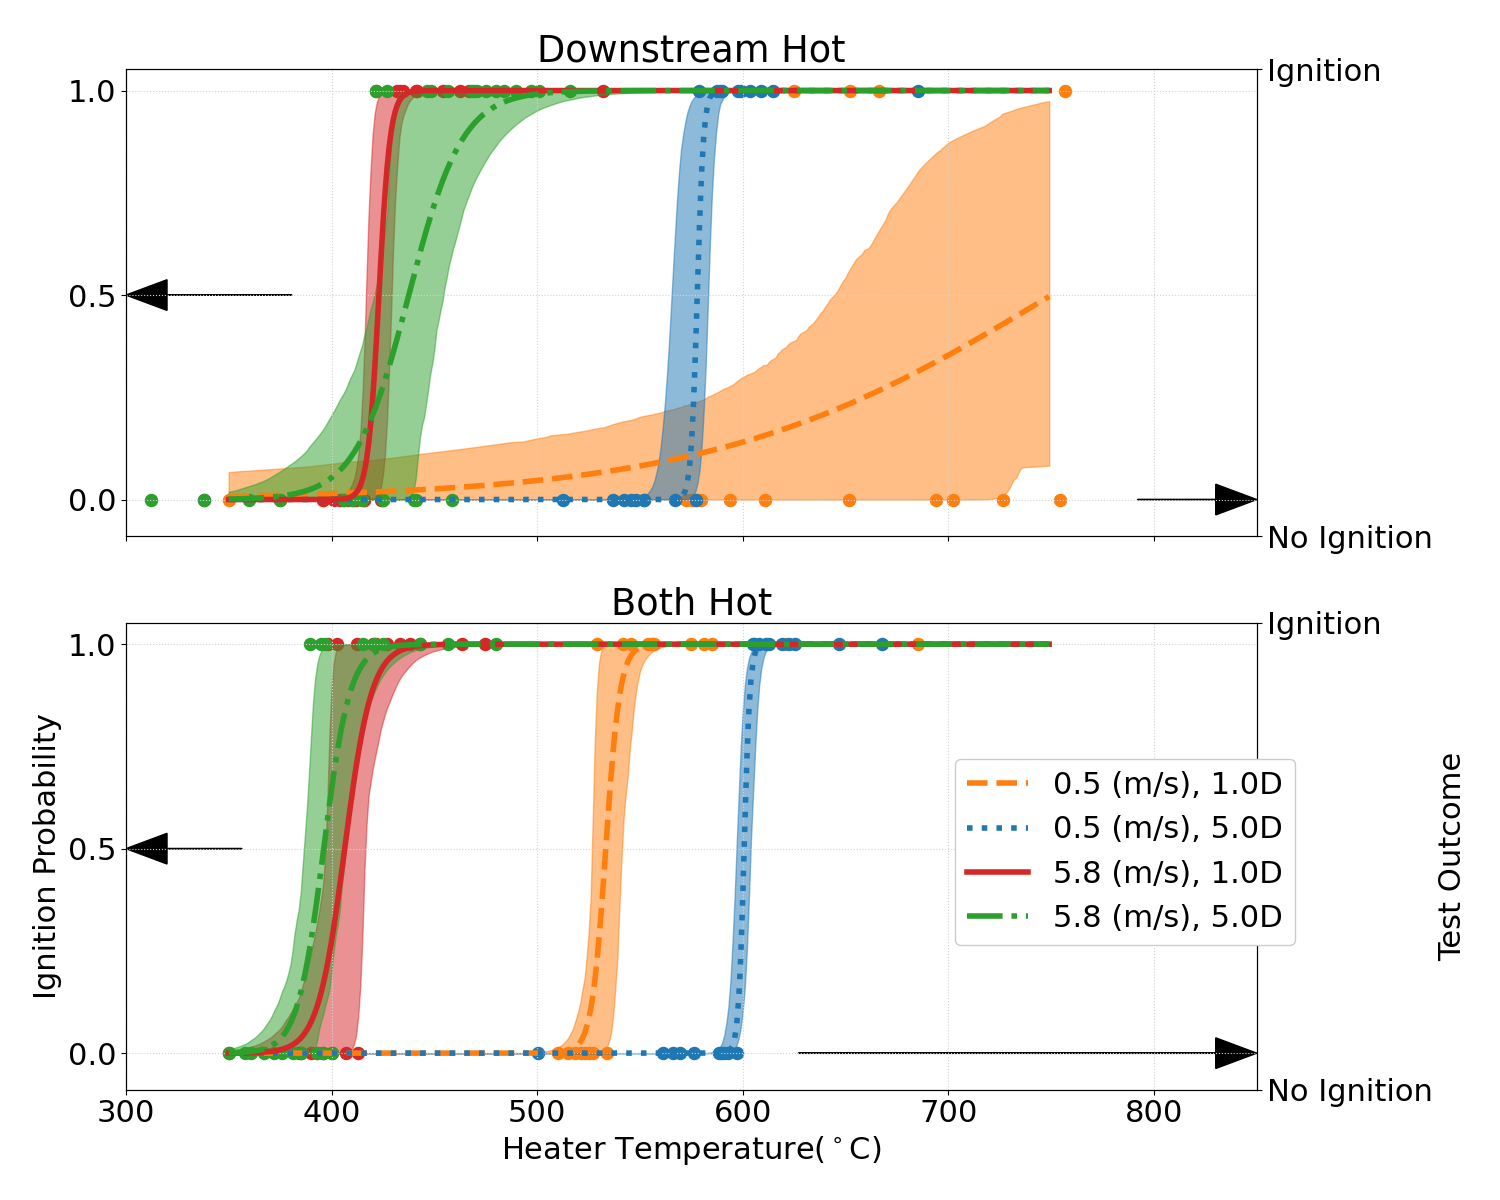
\includegraphics[width=0.75\columnwidth]{Figures/multi_heater_plot.png}
            \caption{Ignition or no ignition outcomes of tests with different heater configurations. The circular markers indicate outcomes of individual tests and the curves represent logistic regressions of each test series. The shaded region shows the 95\% confidence interval for each regression.}
            \label{fig:multi_heater_hot_vs_ambient}
        \end{figure}
    Table~\ref{tab:multiFiftyTemp} shows the heater temperatures estimated to result in a 50\% ignition probability from the logistic regressions shown in Figure~\ref{fig:multi_heater_hot_vs_ambient} with the bounds of the 95\% confidence intervals included. Temperature values for the corresponding wind speed and orientation from the single heater study in Chapter~\ref{part:manuscript2} are shown in the column titled "Single" for comparison. 
        \rowcolors{2}{gray!25}{white}
        \begin{table}[hpbt]
            \normalsize
            \caption{Heater temperature required to achieve 50\% ignition probability for the configurations tested with 95\% confidence intervals shown in parentheses. The single heater column shows the values from the study in Chapter~\ref{part:manuscript2} for a single heater.}
            \centering
            \begin{tabular}{ccrrr}
                \rowcolor{gray!50}
               U\textsubscript{bulk} (\si{\meter\per\second}) & Spacing (D) & Ambient (\si{\celsius})& Heated (\si{\celsius}) & Single (\si{\celsius})\\
                \hline
                0.5  & 1 & 750 (644, 850) & 533 (527, 541) & 571\\
                0.5  & 5 & 578 (565, 583) & 601 (597, 604) & 571\\
                5.8  & 1 & 423 (417, 429) & 406 (397, 416) & 399\\
                5.8  & 5 & 438 (421, 454) & 396 (387, 407) & 399
            \end{tabular}
            \label{tab:multiFiftyTemp}
        \end{table}
        
    Considering first the cases where both heaters are actively heated there are three observations of note. First, in both the one and five heater diameter spacing cases an increase in wind from 0.5\si{\meter\per\second} to 5.8\si{\meter\per\second} resulted in a lower temperature threshold for ignition. These results are consistent with the results for a single heater presented in Chapter~\ref{part:manuscript2} and are attributed to an increased residence time of pyrolyzates near the heater in recirculation zones enabling ignition at lower temperatures. Second, for the 0.5\si{\meter\per\second} wind speed tests decreasing the heater spacing from five heater diameters to one heater diameter resulted in an 11\% decrease in the temperature required for 50\% ignition probability. The shift in ignition probabilities is attributed to increased heat transfer between the closely spaced heaters. For tests that were conducted with heater temperatures near the 50\% ignition temperature a shift in the model of ignition occurred. For cases where the heaters where spaced five diameters apart ignitions occurred within $\approx$1\si{\second} of the heaters being lowered. Similar ignition times were characteristic of the single diameter spaced heaters at higher temperatures. However, for the single diameter spaced heaters ignitions with heater temperatures near the 50\% ignition limit did not typically ignite until the pyrolysis fronts from both heaters merged. Ignition then occurred in the plume of pyrolyzates between the heaters and anchored to the fuel bed. Noting that the ignition threshold for the one diameter spaced heaters is lower than that of the single heater the lower ignition threshold is attributed to the increased heat transfer resulting from two heat sources. It is not clear from these results what specific mechanism is the driving factor. Possibilities include increased temperature of pyrolyzates departing between the heaters due to to enhanced radiative and convective heat transfer, preheating of air as it flows over the upstream heater before mixing, increased mass flux of pyrolyzates from the fuel bed, or a combination of effects. In contrast to the differences in ignition at a wind speed of 0.5\si{\meter\per\second} the differences in ignition probability were not statistically significant at 5.8\si{\meter\per\second}. This suggests that the enhanced heat transfer between the cartridge heaters is not influential in windy conditions. Anecdotally, in cases under wind ignitions were to occur on the upstream side of the upstream cartridge heater suggesting that ignition is more favorable in the recirculation zones on the upstream side of the heater even with the addition of heat and pyrolysis 
   
    Now considering the cases where the only the downstream heater was actively heated there are three observations of note. First, similar to the dual heated and single heater results from Chapter~\ref{part:manuscript2} an increase of wind from an increase of wind from 0.5\si{\meter\per\second} to 5.8\si{\meter\per\second} significantly lowered the ignition threshold. Second, for cases with a wind speed of 5.8\si{\meter\per\second} changing the spacing between the heaters did not have a significant influence on the temperature required for ignition which aligns with the trends observed for the cases where both heaters were hot. Third, decreasing the spacing from five diameters to one diameter in low wind speed conditions increased the temperature required for ignition by greater than 30\% which is opposite trend observed for cases where both heaters were hot. This notable deviation from trends is attributed to the unheated heater acting as a heat sink requiring significantly more energy for ignition. 
    
    More analysis to come. 
    
\section{Conclusions}
    Conclusions for this manuscript will go here. 